\documentclass[11pt]{article}
\usepackage[a4paper,margin=2.3cm]{geometry}
\usepackage[T1]{fontenc}
\usepackage{lmodern}
\usepackage{amsmath}
\usepackage{graphicx}
\usepackage{booktabs}
\usepackage{longtable}
\usepackage{array}
\usepackage{adjustbox}
\usepackage{siunitx}
\usepackage{xcolor}
\usepackage[numbers,sort&compress]{natbib}
\usepackage[hidelinks]{hyperref}
\usepackage{setspace}
\onehalfspacing
% Generated by hwreview.macros - do not edit by hand.
\newcommand{\hwComplMedianPublic}{0.30}
\newcommand{\hwComplMedianSplash}{0.07}
\newcommand{\hwItemBOneAbsent}{1.79}
\newcommand{\hwItemBOneQuant}{98.21}
\newcommand{\hwItemBOneSplashQuant}{46.43}
\newcommand{\hwItemBTwoAbsent}{37.50}
\newcommand{\hwItemBTwoQuant}{33.93}
\newcommand{\hwItemBTwoSplashQuant}{2.68}
\newcommand{\hwItemBThreeAbsent}{90.18}
\newcommand{\hwItemBThreeQuant}{0.00}
\newcommand{\hwItemBThreeSplashQuant}{0.00}
\newcommand{\hwItemEOneAbsent}{47.32}
\newcommand{\hwItemEOneQuant}{29.46}
\newcommand{\hwItemEOneSplashQuant}{12.50}
\newcommand{\hwItemETwoAbsent}{74.11}
\newcommand{\hwItemETwoQuant}{12.50}
\newcommand{\hwItemETwoSplashQuant}{7.14}
\newcommand{\hwItemEThreeAbsent}{58.93}
\newcommand{\hwItemEThreeQuant}{8.04}
\newcommand{\hwItemEThreeSplashQuant}{0.89}
\newcommand{\hwItemEFourAbsent}{85.71}
\newcommand{\hwItemEFourQuant}{10.71}
\newcommand{\hwItemEFourSplashQuant}{4.46}
\newcommand{\hwItemEFiveAbsent}{50.89}
\newcommand{\hwItemEFiveQuant}{11.61}
\newcommand{\hwItemEFiveSplashQuant}{0.00}
\newcommand{\hwItemFOneAbsent}{41.96}
\newcommand{\hwItemFOneQuant}{40.18}
\newcommand{\hwItemFOneSplashQuant}{4.46}
\newcommand{\hwItemFTwoAbsent}{96.43}
\newcommand{\hwItemFTwoQuant}{3.57}
\newcommand{\hwItemFTwoSplashQuant}{0.89}
\newcommand{\hwItemGOneAbsent}{44.64}
\newcommand{\hwItemGOneQuant}{17.86}
\newcommand{\hwItemGOneSplashQuant}{11.61}
\newcommand{\hwItemGTwoAbsent}{30.36}
\newcommand{\hwItemGTwoQuant}{16.96}
\newcommand{\hwItemGTwoSplashQuant}{6.25}
\newcommand{\hwItemGThreeAbsent}{63.39}
\newcommand{\hwItemGThreeQuant}{27.68}
\newcommand{\hwItemGThreeSplashQuant}{9.82}
\newcommand{\hwItemTOneAbsent}{93.75}
\newcommand{\hwItemTOneQuant}{1.79}
\newcommand{\hwItemTOneSplashQuant}{0.00}
\newcommand{\hwItemWOneAbsent}{62.50}
\newcommand{\hwItemWOneQuant}{17.86}
\newcommand{\hwItemWOneSplashQuant}{6.25}
\newcommand{\hwKWCoverageH}{27.69}
\newcommand{\hwKWCoverageN}{112}
\newcommand{\hwKWCoverageP}{9.7\times10^{-7}}
\newcommand{\hwKWEraH}{2.57}
\newcommand{\hwKWEraN}{90}
\newcommand{\hwKWEraP}{0.46}
\newcommand{\hwKWHwClassH}{16.83}
\newcommand{\hwKWHwClassN}{112}
\newcommand{\hwKWHwClassP}{0.00}
\newcommand{\hwKWPlatformH}{30.67}
\newcommand{\hwKWPlatformN}{110}
\newcommand{\hwKWPlatformP}{1.1\times10^{-5}}
\newcommand{\hwKWStatusH}{5.19}
\newcommand{\hwKWStatusN}{112}
\newcommand{\hwKWStatusP}{0.16}
\newcommand{\hwKWUsedH}{27.21}
\newcommand{\hwKWUsedN}{112}
\newcommand{\hwKWUsedP}{1.8\times10^{-7}}
\newcommand{\hwNBioCapable}{164}
\newcommand{\hwNBioWithStudy}{70}
\newcommand{\hwNDatasets}{641}
\newcommand{\hwNDatasetsNoPlatform}{310}
\newcommand{\hwNEntities}{328}
\newcommand{\hwNHabUsed}{34}
\newcommand{\hwNHabitats}{112}
\newcommand{\hwNLinkedStudy}{124}
\newcommand{\hwNNutAgarGel}{11}
\newcommand{\hwNNutAnimalFoodWater}{16}
\newcommand{\hwNNutAquaticWaterLoop}{6}
\newcommand{\hwNNutArcilliteSubstrate}{6}
\newcommand{\hwNNutHydroponicAeroponic}{5}
\newcommand{\hwNNutLiquidCultureMedium}{21}
\newcommand{\hwNNutNoneEvidenced}{60}
\newcommand{\hwNNutWaterOnlyWick}{6}
\newcommand{\hwNPlatAircraftParabolic}{4}
\newcommand{\hwNPlatApolloGemini}{3}
\newcommand{\hwNPlatFreeFlyerBionCosmosBiosatellite}{19}
\newcommand{\hwNPlatIss}{18}
\newcommand{\hwNPlatMir}{3}
\newcommand{\hwNPlatShuttle}{38}
\newcommand{\hwNPlatSkylab}{1}
\newcommand{\hwNPlatSuborbital}{1}
\newcommand{\hwNPlatformNamed}{87}
\newcommand{\hwNPlatformNotHardware}{32}
\newcommand{\hwNPlatformStrings}{116}
\newcommand{\hwNRegistry}{157}
\newcommand{\hwNRoleAnalysisInstrument}{22}
\newcommand{\hwNRoleExperimentUniqueOther}{4}
\newcommand{\hwNRoleExposureFacility}{10}
\newcommand{\hwNRoleGenericOrUnclear}{9}
\newcommand{\hwNRoleGroundAnalog}{4}
\newcommand{\hwNRoleGroundFacility}{23}
\newcommand{\hwNRoleHabitatGrowth}{104}
\newcommand{\hwNRoleHostingFacility}{35}
\newcommand{\hwNRoleNonbio}{21}
\newcommand{\hwNRoleProcessingFixation}{17}
\newcommand{\hwNRoleProgram}{1}
\newcommand{\hwNRoleSensorDosimetry}{37}
\newcommand{\hwNRoleVehicleOrLocation}{14}
\newcommand{\hwNSplash}{147}
\newcommand{\hwNSplashBlock}{27}
\newcommand{\hwNSplashMisattributed}{29}
\newcommand{\hwNSplashUncertain}{6}
\newcommand{\hwNVeggieSpellings}{9}
\newcommand{\hwNuErrRaFiveNOneTwoEight}{0.03}
\newcommand{\hwNuErrRaFiveNSixFour}{0.16}
\newcommand{\hwNuErrRaFiveNNineSix}{0.07}
\newcommand{\hwNuRaFiveNOneTwoEight}{4.52}
\newcommand{\hwNuRaFiveNSixFour}{4.53}
\newcommand{\hwNuRaFiveNNineSix}{4.52}
\newcommand{\hwPUse}{3.3\times10^{-9}}
\newcommand{\hwRhoUse}{0.52}
\newcommand{\hwTierPublicTierA}{1}
\newcommand{\hwTierPublicTierB}{1}
\newcommand{\hwTierPublicTierC}{110}
\newcommand{\hwTierSplashTierA}{0}
\newcommand{\hwTierSplashTierB}{0}
\newcommand{\hwTierSplashTierC}{112}
\newcommand{\hwTierTierLenientA}{9}
\newcommand{\hwTierTierLenientB}{0}
\newcommand{\hwTierTierLenientC}{103}
\newcommand{\hwTierTierWaivefA}{2}
\newcommand{\hwTierTierWaivefB}{7}
\newcommand{\hwTierTierWaivefC}{103}
\newcommand{\hwValAutoExact}{68.89}
\newcommand{\hwValAutoKappa}{0.61}
\newcommand{\hwValAutoMean}{0.36}
\newcommand{\hwValGoldMean}{0.53}
\newcommand{\hwValPrecision}{1.00}
\newcommand{\hwValRaterExact}{90}
\newcommand{\hwValRaterKappa}{0.89}
\newcommand{\hwValRecall}{0.69}
\newcommand{\hwValRho}{0.77}


\title{Which spaceflight biology hardware can be modelled? A metadata audit of NASA's hardware catalogues and three-dimensional transient CFD of specimen environments}
\author{Richard Barker\thanks{ORCID 0000-0001-5681-9857. Correspondence: richard@cosecloud.com.}\\
\small\textbf{[Affiliation and co-authors to be confirmed by the corresponding author]}}
\date{}

\begin{document}
\maketitle

\begin{abstract}
\noindent
Spaceflight biology results are interpreted against the hardware the specimens lived in, yet the
physical environment inside that hardware -- airflow, gas composition, temperature, humidity, light
and nutrient delivery -- is rarely documented well enough to be modelled. We assembled the three
public NASA hardware sources (the SPLASH instrument catalogue, the OSDR hardware registry and the
experiment-platform field of every OSDR study) into \hwNEntities{} hardware entities, of which
\hwNBioCapable{} can carry space-biology payloads and \hwNHabitats{} house live specimens in flight.
We defined a 15-item minimum-information checklist for computational fluid dynamics (CFD) of a
specimen environment, scored every specimen-housing item automatically (validated against two blind
raters; weighted $\kappa=\hwValRaterKappa$ between raters, scorer precision \hwValPrecision{} and
recall \hwValRecall{}) and found that public metadata support a CFD-ready description for
\hwTierPublicTierA{} of \hwNHabitats{} items; SPLASH alone supports none. Airflow rate, specimen
metabolic load and heat load are the least documented inputs. Documentation is better for hardware
that has been used in OSDR studies (Spearman $\rho=\hwRhoUse$) and for ISS-era hardware, and worst for
cell and microbe culture hardware. Curation also exposed catalogue defects, including a block of
\hwNSplashBlock{} SPLASH records whose descriptive fields are displaced from neighbouring rows.
Targeted literature curation, with every value tied to a verbatim source quotation, raised a subset of
heavily used hardware to CFD readiness; for these we built verified three-dimensional transient OpenFOAM
models in flight (0\,$g$) and ground-control (1\,$g$) conditions, with engineering drawings and
four-dimensional field records. In the modelled hardware, gravity changed the specimen-zone CO$_2$ by
\hwCfdMdsGravityDiffPct\% in a ventilated mouse cage and by less than the flow's own fluctuation in a plant
growth chamber, whereas a single undocumented parameter -- the vent size of a passive fly box -- changed the
predicted specimen CO$_2$ \hwCfdVfbCoRatio-fold. The missing metadata, not gravity, dominated the uncertainty
of the modelled environments. All code, data snapshots and curated specifications are released for reuse.
\end{abstract}

\section{Introduction}
Every spaceflight biology experiment is also an experiment on its hardware. Sealed canisters,
fan-ventilated growth chambers, rodent habitats and culture cassettes impose their own gas,
temperature and humidity fields on the specimens, and in microgravity the buoyant convection that
mixes those fields on Earth is absent. When flight and ground-control specimens differ, part of the
difference can therefore arise from the hardware environment rather than from gravity itself. NASA's
Open Science Data Repository (OSDR) now holds hundreds of spaceflight studies \citep{gebre2025,berrios2021},
and the OSDR also publishes two hardware resources: the SPLASH instrument catalogue \citep{splash} and a
hardware registry linked to payloads and studies \citep{osdrapi}. Whether these resources describe the
hardware well enough to reconstruct the specimen environment has not been assessed.

Here we (i) build a crosswalk across the three public hardware sources and count the hardware able to
carry space-biology payloads, where it flies and how it feeds its specimens; (ii) define a minimum
information checklist for CFD of a specimen environment and measure, item by item, how much of it the
public record supplies, validating the automated scoring against blind human-style rating; (iii) run a
meta-analysis of which hardware is under-documented; and (iv) for hardware whose parameters can be
sourced, build verified three-dimensional transient CFD models in 0\,$g$ and 1\,$g$, with orthographic
drawings and time-resolved field records. Throughout, every number either comes from a cited source,
is computed from cited values, or is declared as a modelling assumption.

\section{Methods}
\subsection{Data sources and snapshot}
On 2026-10-12 we downloaded, without authentication, the full SPLASH catalogue
(\nolinkurl{splash-api/public/instruments}, \hwNSplash{} records, 62 fields), the OSDR hardware registry
(\nolinkurl{geode-py/ws/api/hardware}, \hwNRegistry{} records, with every linked payload and experiment
record), and the \texttt{experiment platform}, project identifier and organism of every OSDR dataset
(\hwNDatasets{} datasets) together with each dataset's metadata, including protocol descriptions.
Raw responses are archived with SHA-256 checksums; every downstream stage reads only this snapshot.

\subsection{Catalogue integrity}
Because SPLASH has no structured links, we tested each record's internal consistency before using it.
For each descriptive field we computed TF--IDF cosine similarity between the field and the identity text
(name, alternate names and background) of every record; a field that shared almost nothing with its own
record but matched a record within three rows was flagged as displaced, the signature of a row-offset
error. Organism classes named in the specimen field were also compared with those named in the
record's own background. Every flag was reviewed by hand and given a verdict with a reason and, where
possible, independent evidence from the OSDR registry (Supplementary Table S1).

\subsection{Crosswalk}
SPLASH and registry records were joined into hardware entities by exact match of normalised aliases and
by acronyms unambiguous across both sources; joins that would merge two SPLASH records were refused.
Study platform strings were split into components and mapped many-to-many onto entities (exact alias,
unambiguous acronym or containment of a specific alias), so that a string naming two devices links to
both without merging them. Fuzzy matches were never applied automatically: they were written out as
proposals and accepted or rejected in a curated decision file, each with a reason.

\subsection{Classification}
Each entity was assigned a role (specimen habitat, hosting facility, processing/fixation, analysis
instrument, sensor, exposure facility, ground facility or non-biological) from the SPLASH category
where present, otherwise from keywords in its name and registry description, with curated corrections.
Organism classes were taken from hardware-specific text and from the organisms of linked OSDR studies.
Flight platform was taken from the missions of the hardware's registry payloads. Nutrient and water
delivery modes were assigned only when a verbatim quotation supported them and the mode was compatible
with an organism the hardware carries.

\subsection{Minimum information for CFD (MI-CFD-HW) and its validation}
We defined 15 items needed to model a specimen environment (Supplementary Table S2), six of them
critical: enclosure dimensions, specimen-container dimensions, ventilation mode, airflow rate, specimen
temperature and specimen type. Each item scores 0 (absent), 0.5 (qualitative only) or 1 (quantitative or
explicit), with the quotation that earned the score; laboratory preparation, storage and analysis
sentences are excluded. A hardware item is Tier~A (CFD-ready) when every critical item scores 1, Tier~B
when every critical item scores at least 0.5, and Tier~C otherwise. Two blind raters scored a seeded
random sample of 12 specimen-housing entities (180 cells) from the raw text; disagreements were
adjudicated with written reasons, and the automated scorer was evaluated against the adjudicated gold
standard without further tuning.

\subsection{Meta-analysis}
Completeness (mean item score) was compared across hardware class, flight platform, era, SPLASH status
and catalogue coverage with Kruskal--Wallis tests and pairwise Mann--Whitney tests with
Benjamini--Hochberg correction, and related to the number of OSDR studies using the hardware by
Spearman correlation.

\subsection{Literature curation and audit}
For the \hwNCurated{} specimen-housing hardware items linked to OSDR studies (and their close
relatives), parameters were sought in peer-reviewed papers, NASA technical reports, mission
documentation, vendor pages and the snapshot itself, by five curation passes organised by hardware family.
Each parameter record carries its value, unit, source, URL and a verbatim quotation of at most 40 words;
values were never transferred between hardware items or filled with typical values, unresolved
parameters are left empty with a note of where they were sought, and conflicting sources are recorded
(Supplementary Note~S1). Each pass checked its quotations against saved copies of the sources. An
independent auditor then re-opened the sources of a seeded random sample of \hwNAudit{} records:
\hwNAuditQuoteFound{} quotations were found verbatim and no value was contradicted
(\hwNAuditValueYes{} fully supported; \hwNAuditValuePartial{} supported but with descriptive wording
partly drawn from a second source named in the record's note); three records were corrected.
Tiers after curation use the six critical items, with the airflow requirement waived for sealed or
passive hardware.

\subsection{CFD models}
For Tier~A hardware we generated geometry from parametric primitives (boxes, cylinders, repeated arrays)
in which every number is either a reference to a sourced parameter or a declared modelling assumption
(Supplementary Note~S4); the model loader refuses any other literal. Orthographic
drawings are produced from the same primitives. Meshes were built with \texttt{snappyHexMesh} from a
cubic background mesh whose margin is a non-integer number of cells (so that no background face coincides
with a geometry surface) and solved with \texttt{buoyantBoussinesqPimpleFoam} in OpenFOAM v2606
\citep{weller1998,openfoam2606} with second-order backward time integration. Air properties at the
hardware set-point were computed with CoolProp \citep{bell2014,lemmon2000,lemmon2004} and the aquarium was
modelled with water properties (IAPWS-95 via CoolProp). CO$_2$ (ppm) and water vapour
(mmol\,mol$^{-1}$) were transported as passive scalars with the diffusivities tabulated by
\citet{monteith2008}; specimen fluxes from the curated files were converted to volumetric sources in cell
zones (gas volumes at 0\,$^\circ$C and 1\,atm, 22.414\,L\,mol$^{-1}$), and specimen heat enters the energy
equation. Inlets impose the sourced volumetric flow or face velocity and the supply composition; outlets
fix the pressure; passive vents impose the exterior (ISS cabin) state; gas-permeable membranes use a Robin
condition. The mean age of air was computed with a passive scalar (unit source, zero at inflow). Flow was
treated as laminar: inlet Reynolds numbers (hydraulic diameter) were at most \hwCfdMaxReInletLaminar{} in
all cases except the APH fan-maximum sensitivity case (\hwCfdReInletFanmax{}), which is above transition and
Cases start from the supply state at rest and run until the specimen-zone quantities reach a plateau.
Hardware with a sourced specimen heat load (MDS) was run with gravity off (flight) and on (ground control,
$9.80665$\,m\,s$^{-2}$). Where no heat load could be sourced, the temperature field is uniform and the
Boussinesq model has no buoyancy source, so the 1\,$g$ solution is identical to 0\,$g$ by construction; running
it only admits spurious currents driven by round-off temperature differences, which in a passive,
diffusion-dominated enclosure are not negligible, so these cases were run at 0\,$g$ only. The APH baseline was nevertheless run in both
conditions to show that the difference stays within the temporal fluctuation of the forced flow.

\paragraph{Verification.} The solver configuration was verified on the differentially heated square
cavity against the reference Nusselt numbers of \citet{devahldavis1983} and \citet{hortmann1990} (as
tabulated by \citet{gjesdal2003}) at three Rayleigh numbers on three meshes (mean Nu
\hwNuRaFiveNSixFour{}, \hwNuRaFiveNNineSix{} and \hwNuRaFiveNOneTwoEight{} at
$Ra=10^5$ versus 4.522), on one-dimensional diffusion against the analytic solution, and by closing the
transient CO$_2$ balance (source = outflow + accumulation) in every hardware run. Discretisation
uncertainty of the hardware results was estimated with the grid convergence index \citep{celik2008} on three
meshes (refinement ratio $\sqrt2$) for three hardware items.

\section{Results}
\subsection{The hardware catalogue}
The crosswalk produced \hwNEntities{} entities (\hwNSplash{} in SPLASH, \hwNRegistry{} in the registry);
\hwNPlatformNotHardware{} study platform components named a vehicle, location, ground analogue or
generic item rather than hardware. \hwNBioCapable{} entities can carry space-biology payloads and
\hwNHabitats{} house live specimens during flight (Fig.~\ref{fig:funnel}). Only \hwNHabUsed{} of these are
linked to at least one OSDR study. Mission records place bio-capable hardware on the Space Shuttle
(\hwNPlatShuttle{}), on free-flying biosatellites (\hwNPlatFreeFlyerBionCosmosBiosatellite{}) and on the ISS
(\hwNPlatIss{}). Nutrient delivery was evidenced for fewer than half of the habitats
(\hwNNutNoneEvidenced{} with no evidence); where evidenced, animal food and water
(\hwNNutAnimalFoodWater{}), culture medium (\hwNNutLiquidCultureMedium{}) and agar
(\hwNNutAgarGel{}) were the commonest modes (Fig.~\ref{fig:where}). Every assigned mode is backed by a
verbatim quotation (Supplementary Data, \texttt{T2b\_nutrient\_evidence.csv}).

\begin{figure}[t]\centering
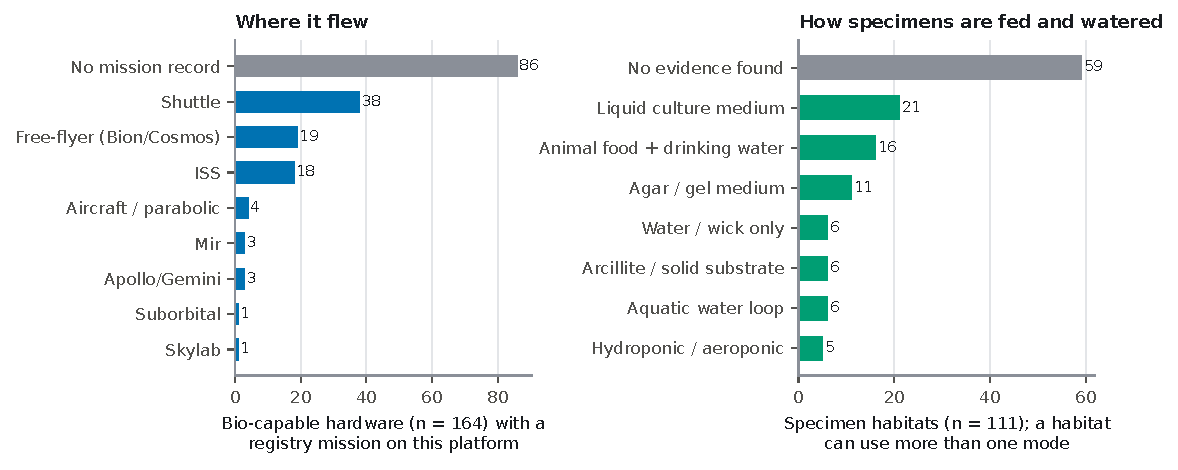
\includegraphics[width=\linewidth]{../results/figures/F8_where_and_feed.pdf}
\caption{Where space-biology hardware flew, from the missions of its registry payloads, and how specimens
in specimen habitats are fed and watered, from quotation-backed evidence.}\label{fig:where}
\end{figure}

\begin{figure}[t]\centering
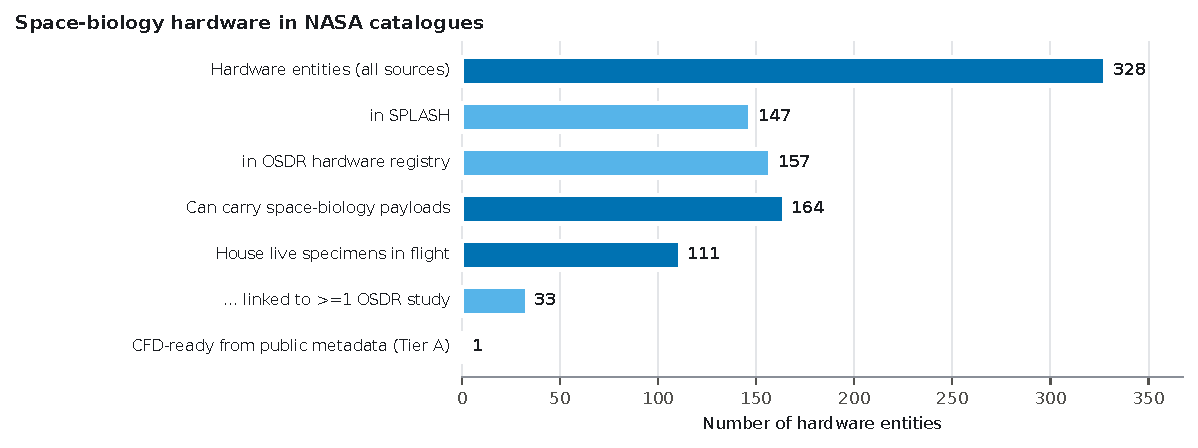
\includegraphics[width=0.85\linewidth]{../results/figures/F1_catalogue_funnel.pdf}
\caption{Space-biology hardware in the three NASA sources, from all entities to those whose public
metadata support a CFD model.}\label{fig:funnel}
\end{figure}

\subsection{Catalogue defects}
\hwNSplashBlock{} SPLASH records (\#121--\#147) carry descriptive fields displaced from neighbouring rows:
\hwNSplashMisattributed{} fields were confirmed as misattributed on review, for example a Plant Growth Unit
record whose specimen field describes an RNA thermal cycler, and a BRIC-Opti canister record carrying
the crop list and CO$_2$, humidity and temperature control ranges of the Advanced Plant Habitat. The
\texttt{sources}, \texttt{schematics} and \texttt{study\_links} fields are empty in every record.
\hwNDatasetsNoPlatform{} of \hwNDatasets{} OSDR datasets have no experiment-platform entry; the remainder
use \hwNPlatformStrings{} free-text strings, with \hwNVeggieSpellings{} spellings of Veggie alone.

\subsection{How much of a CFD model the public record supplies}
Specimen type is almost always stated (\hwItemBOneQuant\% quantitative), but airflow rate
(\hwItemFTwoQuant\%), specimen metabolic load (\hwItemBThreeQuant\%) and heat load (\hwItemTOneQuant\%)
are almost never given (Fig.~\ref{fig:items}). Median completeness was \hwComplMedianPublic{} using all
public sources and \hwComplMedianSplash{} using SPLASH alone. \hwTierPublicTierA{} of \hwNHabitats{}
specimen-housing items reached Tier~A from public metadata and \hwTierSplashTierA{} from SPLASH alone;
waiving the airflow requirement for sealed or passive hardware raised this to \hwTierTierWaivefA{}.
Blind raters agreed on \hwValRaterExact\% of 180 cells (weighted $\kappa=\hwValRaterKappa$). Against the
adjudicated gold standard the automated scorer never credited absent information (precision
\hwValPrecision) but missed some (recall \hwValRecall; mean completeness \hwValAutoMean{} versus
\hwValGoldMean{} gold), so automated completeness is a conservative lower bound; no sampled entity was
Tier~A on the gold scores either.

\begin{figure}[t]\centering
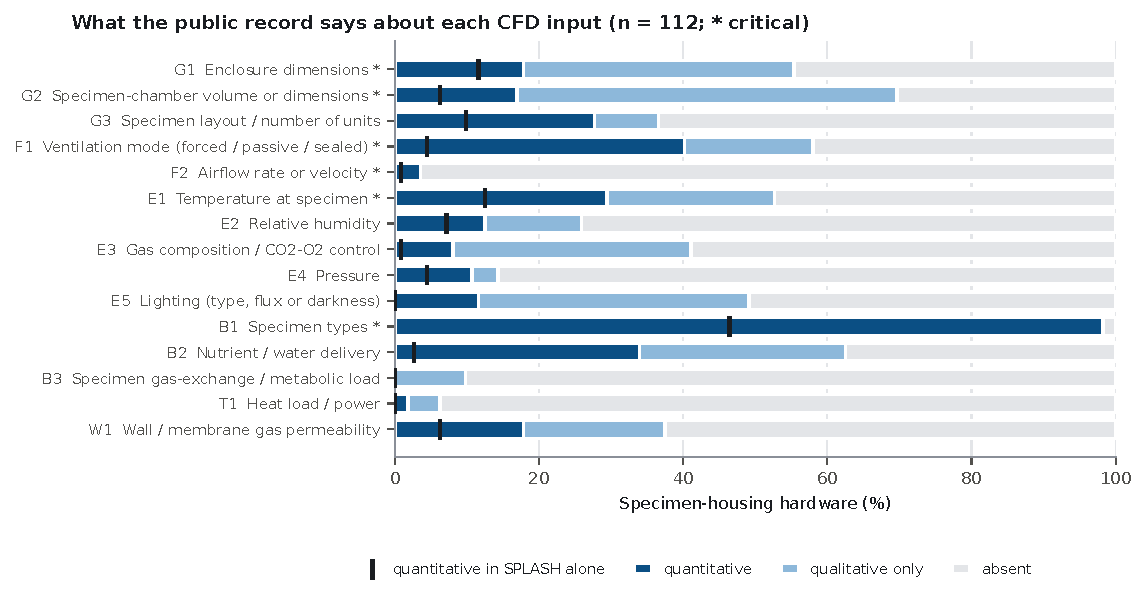
\includegraphics[width=0.9\linewidth]{../results/figures/F2_item_coverage.pdf}
\caption{Coverage of each MI-CFD-HW item across specimen-housing hardware. Dark: quantitative; light:
qualitative only; grey: absent. Ticks: quantitative in SPLASH alone.}\label{fig:items}
\end{figure}

\subsection{Which hardware is under-documented}
Completeness differed by hardware class (Kruskal--Wallis $p=\hwKWHwClassP$), flight platform
($p=\hwKWPlatformP$) and catalogue coverage ($p=\hwKWCoverageP$), but not by era ($p=\hwKWEraP$) or SPLASH
status ($p=\hwKWStatusP$) (Fig.~\ref{fig:groups}). Cell and microbe culture hardware was least documented
and ISS hardware best. Hardware used in OSDR studies was better documented than unused hardware
($p=\hwKWUsedP$; $\rho=\hwRhoUse$ with the number of studies, Fig.~\ref{fig:usage}), but several used
items remain below the median.

\begin{figure}[t]\centering
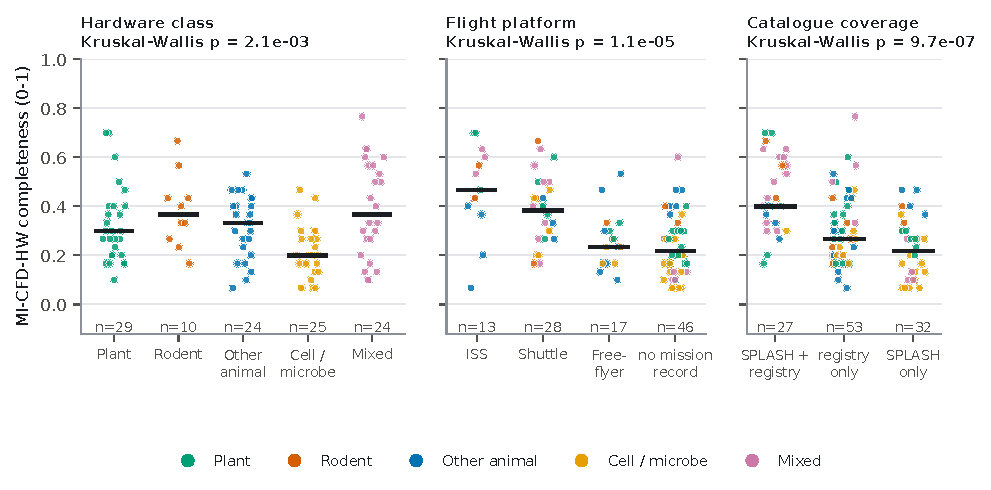
\includegraphics[width=\linewidth]{../results/figures/F3_completeness_groups.pdf}
\caption{MI-CFD-HW completeness by hardware class, flight platform and catalogue coverage (bars:
medians).}\label{fig:groups}
\end{figure}

\begin{figure}[t]\centering
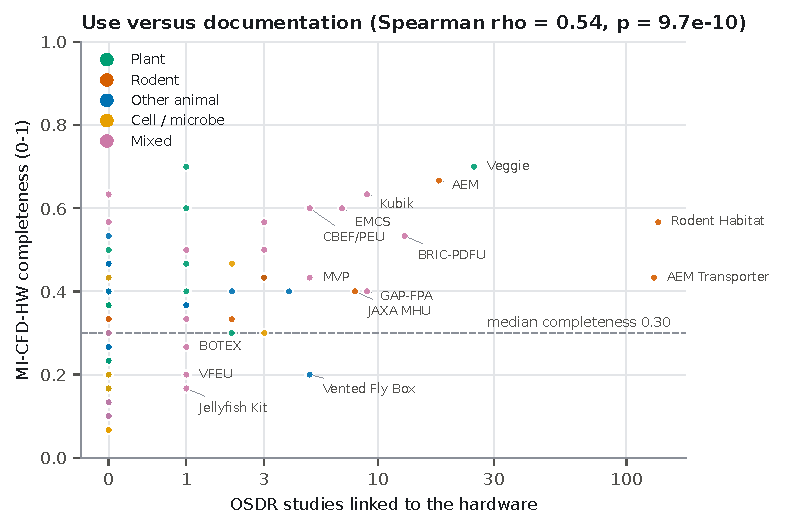
\includegraphics[width=0.75\linewidth]{../results/figures/F4_usage_vs_completeness.pdf}
\caption{Documentation versus scientific use. Points: specimen-housing hardware.}\label{fig:usage}
\end{figure}

\subsection{Literature curation}
Curation of \hwNCurated{} hardware items yielded \hwNCuratedSourced{} sourced parameters out of
\hwNCuratedParams{} sought (\hwPctCuratedSourced\%). \hwNCuratedA{} items reached Tier~A (the Advanced Plant
Habitat, the JAXA Aquatic Habitat, the Mice Drawer System and the Vented Fly Box), \hwNCuratedB{} remained
Tier~B and \hwNCuratedC{} Tier~C (Fig.~\ref{fig:curated}; Supplementary Note~S3).

\begin{figure}[t]\centering
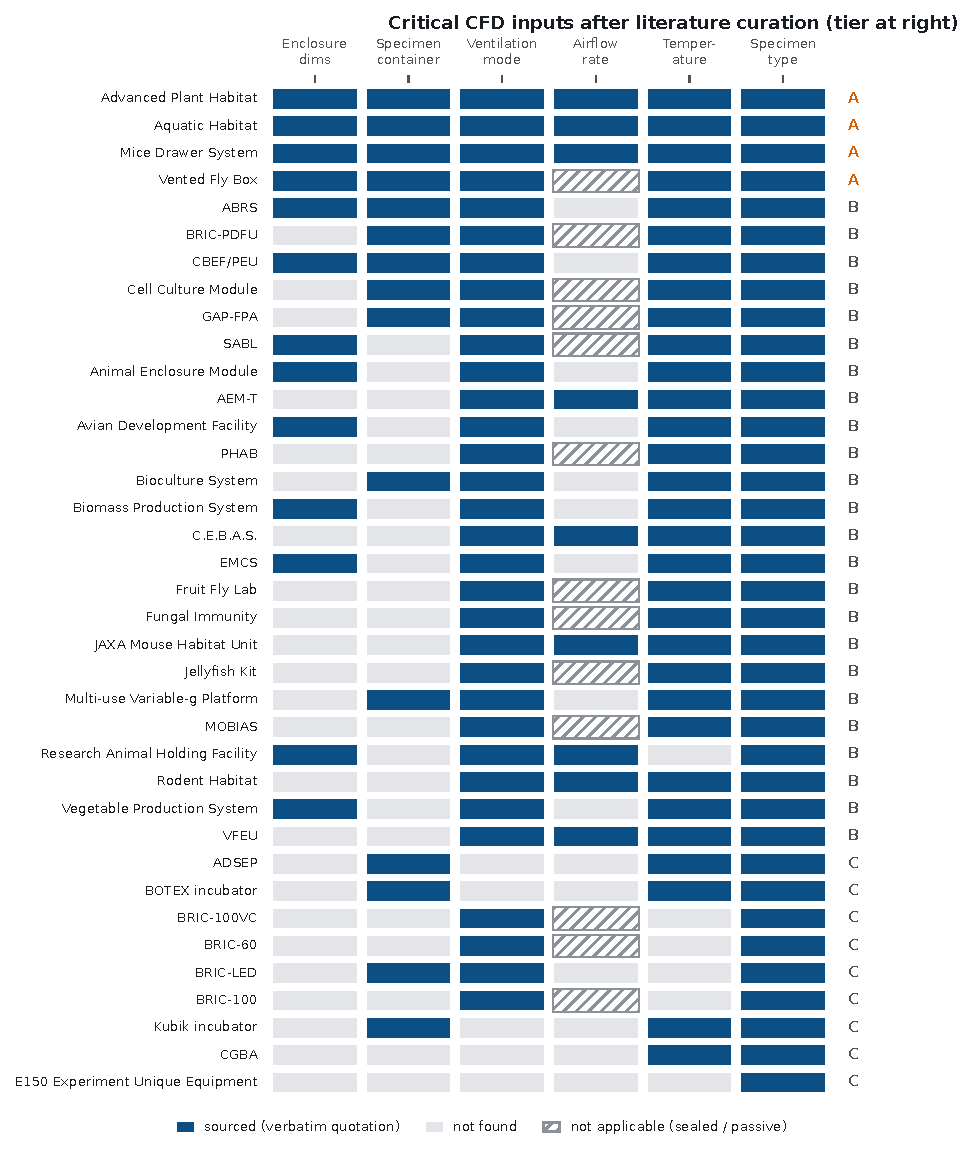
\includegraphics[width=0.78\linewidth]{../results/figures/F7_curated_gaps.pdf}
\caption{Critical CFD inputs for the \hwNCurated{} curated hardware items after literature curation.}
\label{fig:curated}
\end{figure}

\subsection{Verification}
The solver reproduced the reference heated-cavity Nusselt numbers with second-order convergence
(observed order \hwVerPRaFive{} and \hwVerPRaSix{} at $Ra=10^5$ and $10^6$); Richardson-extrapolated values
were within \hwVerMaxExtErr\% of \citet{hortmann1990} (Table~\ref{tab:verify}). One-dimensional diffusion
matched the analytic solution to $\hwVerDiffMaxErr$ (concentration scale 0--1), and the transient CO$_2$
balance closed to within \hwCfdMaxImbalance\% in every hardware run.

\begin{table}[htbp]\centering\footnotesize
\caption{Verification on the differentially heated cavity (Pr 0.71): mean wall Nusselt number on three meshes, observed order $p$, Richardson-extrapolated value and its error against \citet{hortmann1990}.}\label{tab:verify}
\begin{tabular}{ccccccccl}
\toprule
$Ra$ & Nu $64^2$ & Nu $96^2$ & Nu $128^2$ & $p$ & Nu$_{ext}$ & Ref. & Err. (\%) & Convergence \\
\midrule
$10^{4}$ & 2.2447 & 2.2447 & 2.2434 & 15.84 & 2.2434 & 2.245 & -0.071 & oscillatory \\
$10^{5}$ & 4.5293 & 4.5250 & 4.5235 & 2.05 & 4.5217 & 4.522 & -0.007 & monotonic \\
$10^{6}$ & 8.8829 & 8.8496 & 8.8386 & 2.15 & 8.8257 & 8.825 & +0.008 & monotonic \\
\bottomrule
\end{tabular}
\end{table}


\subsection{Specimen environments in flight and ground control}
Table~\ref{tab:cfd} and Fig.~\ref{fig:cfdcomp} summarise the specimen environments at the end of each run;
field slices, environment cards and animations are in the Supplementary Information.

\paragraph{Mice Drawer System.} With the sourced cage through-flow (0.2--0.3\,m\,s$^{-1}$) and organism-level
loads for a 30\,g mouse, the air around the mouse carried \hwCfdMdsZeroCo{}\,ppm more CO$_2$ than the supply,
was \hwCfdMdsZeroDt{}\,K warmer and had a mean age of \hwCfdMdsZeroAge{}\,s. Flight and ground control
differed by \hwCfdMdsGravityDiffPct\% in CO$_2$ excess: at a Richardson number of \hwCfdMdsZeroRi{} the
forced flow dominates the mouse's buoyant plume. The mouse-zone CO$_2$ excess converged monotonically with
mesh refinement (observed order \hwGciPMdsCo{}, fine-mesh GCI \hwGciMdsCo\%).

\paragraph{Advanced Plant Habitat.} At the PH-04 set-points the canopy drew CO$_2$ down by
\hwCfdAphZeroCo{}\,ppm relative to the 550\,ppm supply in flight (temporal s.d.\ \hwCfdAphZeroCoSd{}\,ppm) and by
\hwCfdAphOneCo{}\,ppm in ground control (s.d.\ \hwCfdAphOneCoSd{}\,ppm), a difference of
\hwCfdAphGravityDiff{}\,ppm that lies within the fluctuation of the transitional, fan-driven flow; with no
sourced canopy or lamp heat load the Boussinesq model has no buoyancy source. The mean age of canopy air
was \hwCfdAphZeroAge{}\,s in flight and \hwCfdAphOneAge{}\,s in ground control, and mesh-to-mesh differences
were smaller than the temporal fluctuation (Supplementary Table~S5). Setting the
fans to their maximum speed changed the canopy CO$_2$ drawdown to \hwCfdAphFanmaxZeroCo{}\,ppm and the canopy
age of air to \hwCfdAphFanmaxZeroAge{}\,s (laminar approximation).

\paragraph{Vented Fly Box.} The box exchanges gas with the cabin only through its vents, whose size is not
published. With 20\,mm vents the CO$_2$ excess at the vial plugs reached \hwCfdVfbSmallZeroCo{}\,ppm, with
60\,mm vents \hwCfdVfbLargeZeroCo{}\,ppm: the undocumented vent size alone changes the predicted specimen
CO$_2$ \hwCfdVfbCoRatio-fold and the time to reach 90\% of the plateau \hwCfdVfbTninetyRatio-fold
(\hwCfdVfbSmallZeroTninety{} versus \hwCfdVfbLargeZeroTninety{}\,s). Because the fly load contributes no
sourced heat, the model has no thermal buoyancy; the solutal Rayleigh number of the CO$_2$ excess, which
the model omits, was \hwCfdVfbSmallZeroRaSol{} and \hwCfdVfbLargeZeroRaSol{} for the two vent sizes,
so density-driven exchange in a 1\,$g$ ground control remains a candidate gravity effect that these
metadata cannot resolve.

\paragraph{Aquatic Habitat.} At the sourced 0.1\,L\,min$^{-1}$ per aquarium, the mean age of water in the
aquarium was \hwCfdAqhZeroAge{}\,s against a nominal residence time of \hwCfdAqhZeroTau{}\,s; a mean age
above the nominal residence time indicates poorly flushed regions for the assumed port positions.

\begin{table}[htbp]\centering\scriptsize
\caption{Specimen-environment results (medium mesh, end of run): excess over the supply/initial state in the specimen zone, its age of air, peak velocity, Reynolds and Richardson numbers, and the relative closure of the transient CO$_2$ balance.}\label{tab:cfd}
\begin{tabular}{lllrrrrrrrr}
\toprule
Model & $g$ & Zone & $\Delta$CO$_2$ (ppm) & $\Delta$H$_2$O (mmol/mol) & $\Delta T$ (K) & Age (s) & $U_{max}$ (m/s) & Re & Ri (1 g) & CO$_2$ imbalance \\
\midrule
MDS mouse cage & 0g & mouse & 15.18 & 0.06 & 0.287 & 0.27 & 0.309 & 1932 & $9.67\times10^{-3}$ & $-2.00\times10^{-7}$ \\
MDS mouse cage & 1g & mouse & 15.21 & 0.06 & 0.287 & 0.27 & 0.309 & 1932 & $9.69\times10^{-3}$ & $-2.00\times10^{-7}$ \\
\bottomrule
\end{tabular}
\end{table}


\begin{figure}[t]\centering
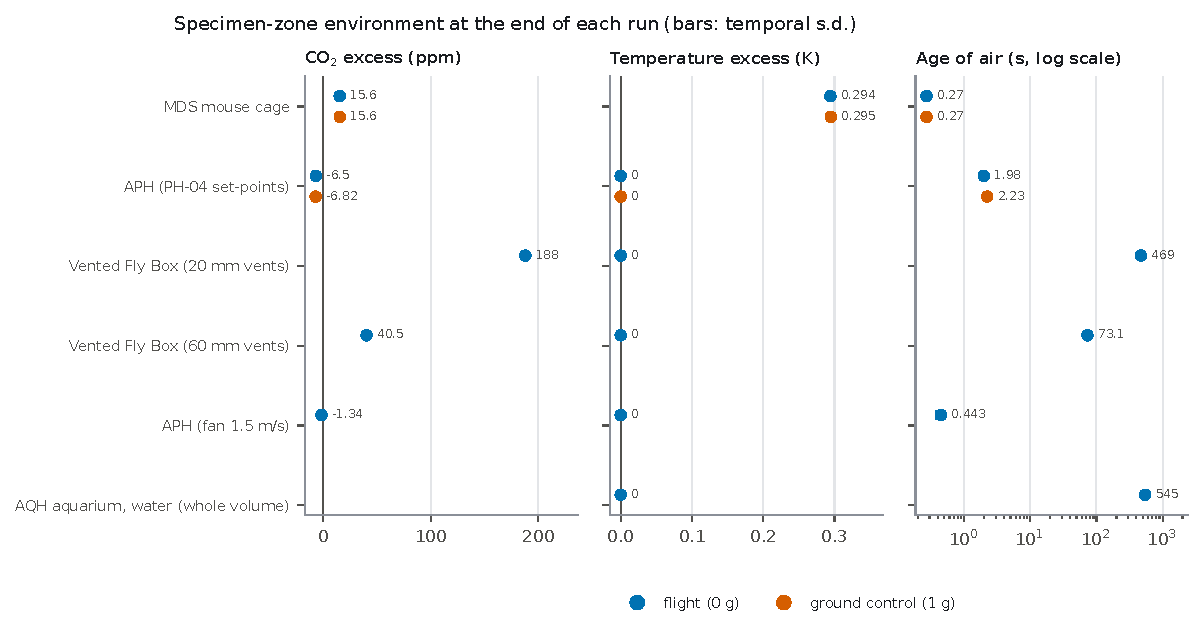
\includegraphics[width=\linewidth]{../results/figures/F6_cfd_comparison_medium.pdf}
\caption{Specimen-zone CO$_2$ and temperature excess and age of air in each modelled hardware item, flight
(0\,$g$) versus ground control (1\,$g$), medium meshes.}\label{fig:cfdcomp}
\end{figure}

\section{Discussion}
\subsection{The specimen environment is mostly undocumented}
Of \hwNHabitats{} hardware items that house live specimens in flight, the public record supports a CFD
description of \hwTierPublicTierA{}, and SPLASH alone supports none. Targeted curation of \hwNCurated{} items,
reading papers, technical reports and mission documentation, raised only \hwNCuratedA{} to CFD readiness.
The single most common gap is the airflow that ventilates the specimens: it is missing for
\hwNMissingFTwo{} curated items, including Veggie (whose fan is described only by its Low/High/Off
settings), EMCS, ABRS and the Biomass Production System. The second is the geometry of the specimen
container and of the enclosure itself. The ISS Rodent Habitat, linked to \hwNStudiesRodentHabitat{} OSDR
studies, has no published internal cage dimensions in any source we could open, and the dimensions of its
predecessor, the Animal Enclosure Module, cannot be assumed to carry over. None of the nine canister and culture items of the BRIC family,
GAP-FPA, BioCell, Kubik and CGBA has published internal dimensions, although BRIC-PDFU alone is linked to
\hwNStudiesBricPdfu{} OSDR studies. Specimen metabolic and heat loads are almost
never reported for the flight itself and had to be taken from organism-level physiology. These are not
obscure parameters: they set the gas, temperature and humidity fields that flight and ground-control
specimens experience, and they are exactly what is needed to judge whether a flight--ground difference is
a gravity effect or a hardware effect.

\subsection{What the models can and cannot say}
In the four hardware items that could be modelled, the gravity contrast was small: forced ventilation
dominated the mouse-cage environment, and in the plant growth chamber the flight--ground difference was
within the fluctuation of the flow. This is not evidence that gravity does not matter to these
environments, because the loads that would let it act -- canopy and lamp heat, fly metabolic heat, the
solutal buoyancy of exhaled CO$_2$ -- are exactly the inputs the public record does not provide. What the
models do show is that the undocumented inputs can matter more than gravity: the fly-box vent size, which
no source states, changed the predicted CO$_2$ around the specimens \hwCfdVfbCoRatio-fold. For hardware of
this kind, interpreting a flight--ground difference as a gravity effect requires the hardware environment
to be measured or modelled, and modelling requires metadata that do not yet exist publicly.

\subsection{Catalogue integrity}
The defects we found are of a kind that propagates silently: displaced fields in a contiguous block of
SPLASH records (a plant growth unit described by an RNA thermal cycler's specimen list, a sealed canister
carrying a growth chamber's CO$_2$ control range), an alias that merges two different bioreactors, and
registry links that attach unrelated studies to hardware. Automated reuse of these catalogues -- including
by language models -- would inherit the errors. We therefore recommend that SPLASH and the OSDR registry
(i)~adopt the MI-CFD-HW items as structured fields with units and provenance, (ii)~populate the existing but
empty \texttt{sources}, \texttt{schematics} and \texttt{study\_links} fields, (iii)~replace the free-text
experiment-platform field of OSDR studies with a controlled reference to a hardware identifier, and
(iv)~record, per flight, the logged temperature, humidity and CO$_2$ of the hardware interior.

\subsection{Limitations}
The automated scorer is conservative (recall \hwValRecall{}) and its tiers are a lower bound; the blind gold
standard, however, also contained no Tier~A item. Curation was bounded by access: several sources likely to
hold the missing airflow and geometry data were paywalled or unavailable and are listed in the curation notes.
The CFD models are laminar and Boussinesq in temperature only; solutal buoyancy from CO$_2$ and water vapour
is not simulated, and we report its Rayleigh number for each run instead. Where heat loads were not sourced
(plant canopies, LED arrays, flies) they were not invented, so buoyancy in the 1\,$g$ cases is driven only by
the sourced loads and gravity contrasts are lower bounds. Unpublished details -- vent sizes and positions,
canopy height, the location at which a fan's ``wind speed'' is measured -- are declared assumptions
(Supplementary Note~S4) and, where they matter, were varied.

\section*{Data and code availability}
Code, the 2026-10-12 source snapshot, curated hardware specifications, model definitions, reduced CFD
outputs and this manuscript's sources are archived on Zenodo (DOI to be assigned on deposit) under the
MIT licence (code) and CC-BY-4.0 (data and figures). SPLASH data were obtained from NASA's Space Life
Sciences Archive of Scientific Hardware \citep{splash}.

\bibliographystyle{unsrtnat}
\bibliography{references}
\end{document}
